\section{Obrzęd Komunii Św.}

\begin{itemize}
      \item \zz~ przynosi {\color{violet} fioletową} stułę, ornat i manipularz,
            odnosi stułę czarną
      \item \ii~ zmienia szaty w asyście \cc1
      \item \ii, \cc1, \cc2, \aa1, \aa2, \kolatki1 i \kolatki2, \oo~ oraz
            pozostali ministranci ustawiają się przed stopniami ołtarza,
            przyklękają i procesyjnie odchodzą krótką drogą do ołtarza
            przechowania

            \newpage

            \begin{center}
                  (stopnie ołtarza) \smallskip\\
                  \cc2~~\ii~~\cc1 \smallskip\\
                  \aa2~~~~\aa1 \smallskip\\
                  \kolatki2~~~~\kolatki1 \smallskip\\
                  ministranci w parach \smallskip\\
                  \oo \smallskip\\
                  \downarrow
            \end{center}

      \item do kaplicy przechowania wchodzą wyłącznie \ii, \cc1, \cc2, \tt1 i
            \tt2; kaplicy następuje zasypanie i okadzenie
      \item wyznaczeni ministranci z pomocą \zz~ zapalają pochodnie na zewnątrz
            kaplicy
      \item \cc2 nakłada \ii~ biały welon, \aa1 i \aa2 biorą zapalone
                  {\color{orange}żółte} świece, \oo~ bierze ombrelino, \ding{63}
            bierze krzyż procesyjny, \kolatki1 i \kolatki2 biorą kołatki
      \item \ii~ niesie Najświętszy Sakrament (cyborium i dużą Hostię), \kolatki1 i
            \kolatki2 uderzają kołatkami i procesyjnie wracają do ołtarza dłuższą
            drogą

            \begin{center}
                  \uparrow \smallskip\\
                  \aa2~~\ding{63}~~\aa1 \smallskip\\
                  ministranci \smallskip\\
                  \kolatki2~~\kolatki1 \smallskip\\
                  \tt2~~\tt1 \smallskip\\
                  pochodnie~~\cc2~~\ii~~\cc1 pochodnie \smallskip\\
                  \oo
            \end{center}

      \item przy zwężeniu pochodnie idą w dwóch szeregach jak pozostali
            uczestnicy procesji; podążają wówczas przed \tt\tt
      \item gdy procesja wraca z NS, wszyscy \textbf{klękają}, schola w tym
            czasie śpiewa hymn \textit{Vexilla Regis}
      \item po dojściu do stopni ołtarza :
            \begin{itemize}
                  \item \aa1 i \aa2 wstępują po stopniach, zostawiają drugą parę
                        świec, po czym wracają do kredensji, gdzie \aa1 zapala
                        obie przygotowane świeczki \textit{sanctusowe} i zanosi
                        jedną na ołtarz,
                  \item ministranci oraz \kolatki1 i \kolatki2
                        wracają na swoje miejsca i klękają
                  \item \tt1 i \tt2 idą na prawo i klękają
                  \item \ii~ wstępuje po stopniach
                  \item \cc1 i \cc2 rozchodzą się na boki
                  \item pochodnie ustawiają się w dwóch rzędach nieco dalej od
                        ołtarza, twarzą do siebie i tak klękają
                  \item \oo~ odstawia ombrelino za ołtarz i wraca na swoje
                        miejsce
            \end{itemize}

            \begin{figure}[h]
                  \centering
                  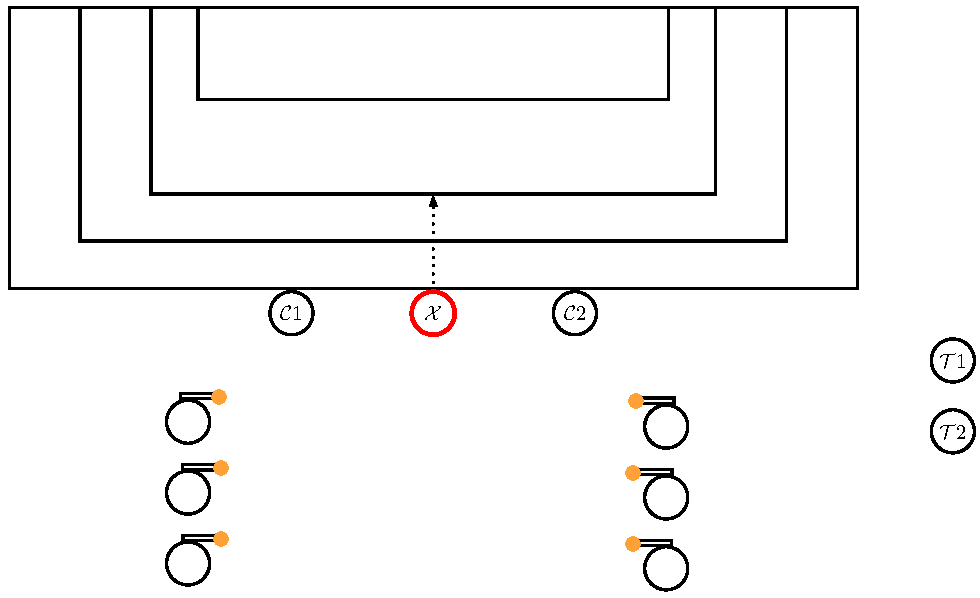
\includegraphics[scale=0.55]{Piatek/NSakrament.pdf}
                  \caption{Procesja po przybyciu do ołtarza}
            \end{figure}

      \item \ii~ odstawia Najświętszy Sakrament, przyklęka i schodzi przed
            stopnie, gdzie \cc2 odbiera od niego welon naramienny.
      \item następuje zasypanie i okadzenie, po którym \tt1 i \tt2 odnoszą
            kadzielnice, wracają do Komunii (po \textit{Pater noster})
      \item \cc1 i \ii~ wchodzą na stopnie, \cc1 asystuje przy mszale
      \item wszyscy ministranci klęczą
      \item \ii~ w tonie ferialnym intonuje \textit{Pater noster} i śpiewa sam.
            Lud odpowiada: \textit{Sed libera nos...}
      \item na znak \cc3 ministranci wstają i ustawiają się parami na środku, na
            początku duchowieństwo, potem \cc1 z \cc2, \aa1 z \aa2, za nimi inni
            ministranci

            \begin{center}
                  (stopnie ołtarza) \smallskip\\
                  duchowieństwo \smallskip\\
                  \cc2~~\cc1 \smallskip\\
                  \aa2~~\aa2 \smallskip\\
                  ministranci
            \end{center}

      \item \cc2 zabiera patenę z kredencji
      \item na znak \cc3 wszyscy przyklękają, pierwsza para ministrantów (lub,
            jeśli jest, pierwsza para duchowieństwa) wchodzą na najwyższy stopień
            ołtarza
      \item na kolejny znak wszyscy klękają
      \item gdy \ii~ odmawia \textit{Domine, non sum dignus} \cc3 uderza w
            kołatkę (trzykrotnie)
      \item po komunii \ii, \cc2 rozpoczyna \textit{Confiteor}, który recytują
            głośno wszyscy obecni
      \item po \textit{Indulgentiam} \cc2 podaje patenę pierwszemu duchownemu
      \item \cc1 i \cc2 asystują X przy Komunii.
      \item \aa1 i \aa2 po przyjęciu Komunii biorą drugą patenę i świeczkę i
            razem z drugim kapłanem udają się do kaplicy po cyborium, a
            następnie asystują mu w udzielaniu Komunii św.
      \item \tt1 i \tt2 wychodzą przygotować kadzidło
      \item pozostali ministranci klęczą
      \item po Komunii \ii~ oczyszcza patenę, którą zabiera A1
      \item gdy NS zostanie schowany, wszyscy \textbf{wstają}, pochodnie wracają
            do poprzedniej pozycji (tzn. rzędem skierowani twarzą do ołtarza)
      \item \ii~ śpiewa trzy oracje, zebrani odpowiadają \textit{Amen}
      \item \zz~ przynosi fioletową kapę
      \item \ii~ zamyka mszał, schodzi ze stopni i razem z \cc1 przyklęka na
            środku i udaje się do sedilli
      \item \ii~ z pomocą \cc1 i \cc2 zdejmuje ornat i manipularz, zakłada kapę
      \item \zz~ odnosi ornat
\end{itemize}

